\def\nr{4. Aufgabenblatt}
\def\kopf{\\\hfill\normalsize\mdseries}
\documentclass[11pt,a4paper,fleqn]{scrartcl}
\usepackage{eurosym}
%\usepackage{a4kopka}
\usepackage{amsmath,amssymb,amsthm,amsfonts}
\usepackage[utf8]{inputenc}
\usepackage{algorithmic,algorithm}
\usepackage{graphics,graphicx}
\usepackage{pgfplots,tikz}
\usepackage{enumerate}
\usepackage[ngerman]{babel}
% \usepackage[software]{mymacros}
%\usepackage{matrix}
\usepackage{hyperref}
% \usepackage{caption}
\usepackage{caption, subcaption}

\floatname{algorithm}{Algorithmus}
\renewcommand{\algorithmicrequire}{\textbf{Input:}}
\renewcommand{\algorithmicensure}{\textbf{Output:}}

%\usepackage{enumitem} 
%\textheight25cm
\textheight23cm
\topmargin-15mm
\oddsidemargin-5mm    %  -10mm
\textwidth17cm    %   18.8cm
\footskip0pt
\thispagestyle{empty}
\parindent0mm
\parskip0ex
\parskip0ex

\makeatletter
\DeclareOldFontCommand{\rm}{\normalfont\rmfamily}{\mathrm}
\DeclareOldFontCommand{\sf}{\normalfont\sffamily}{\mathsf}
\DeclareOldFontCommand{\tt}{\normalfont\ttfamily}{\mathtt}
\DeclareOldFontCommand{\bf}{\normalfont\bfseries}{\mathbf}
\DeclareOldFontCommand{\it}{\normalfont\itshape}{\mathit}
\DeclareOldFontCommand{\sl}{\normalfont\slshape}{\@nomath\sl}
\DeclareOldFontCommand{\sc}{\normalfont\scshape}{\@nomath\sc}
\makeatother

% \newcommand{\cg}[1]{{\color{blue} #1}}
% \newcommand{\cb}[1]{{\color{green} #1}}
% \newcommand{\cred}[1]{{\color{red} #1}}
% \newcommand{\cc}[1]{{\color{cyan} #1}}
% \newcommand{\cm}[1]{{\color{magenta} #1}}

\newcommand{\Aufgabe}[2][]{\par\bigskip{\sf\bfseries Aufgabe #2#1:}}
%\hspace{3em}{\small(#2 point\ifthenelse{#2>1}{s}{})}}\par\smallskip}
%\newcommand\aufgabe[2][~]{\par\bigskip{\sf\bfseries Aufgabe #1
%    \hspace{3em} \ifthenelse{\equal{#2}{~}}{}{(#2)}}\par\smallskip}
\usepackage{mymacros}

\begin{document}
{\sf Universit\"at Hamburg \hfill Wintersemester 2020/21 \\ Fachbereich Mathematik \\ Dr. Matthias Voigt}
\begin{center}
\ifthenelse{\equal{\nr}{no}}{\Large\sf\bfseries \kopf}{\Large\sf\bfseries Optimierung f\"ur Studierende der Informatik -- \nr.~\kopf}
\end{center}

\renewcommand{\tilde}{\widetilde}
\renewcommand{\hat}{\widehat}
\newcommand{\ri}{\mathrm{i}}
\renewcommand{\H}{\mathsf{H}}
\newcommand{\T}{\mathsf{T}}


\subsection*{Präsenzaufgaben am 30.11./01.12.2020}

\Aufgabe[ (Energieflussprobleme)]{P1}
Im Beispiel {\glqq}Energieflussproblem{\grqq} in Abschnitt 6.2 des Skripts wird erläutert, wie das Problem eines \emph{Flusses maximaler Stärke} als LP-Problem formuliert werden kann. Beantworten Sie hierzu die folgenden Fragen:
\begin{enumerate}[a)]
% Aufgabe P-1a
\item Wie viele Variablen gibt es in diesem LP-Problem?
% Aufgabe P-1b
\item Wie lautet die Nebenbedingung, die zum Knoten $V_6$ gehört?
% Aufgabe P-1c
\item Wie viele Nebenbedingungen gibt es insgesamt? (Die Nichtnegativitätsbedingungen sollen nicht mitgezählt werden.)
% Aufgabe P-1d
\item Wie lautet die Zielfunktion?
\end{enumerate}

\Aufgabe[ (Flüsse maximaler Stärke)]{P2}
Anstelle des Netzwerks aus Aufgabe P1 betrachten wir nun das folgende Flussnetzwerk ($v_0$ bezeichnet die \textit{Quelle}, $v_3$ die \textit{Senke} und die Zahlen an den Kanten geben die \textit{Kapazitäten} an):

\begin{center}
 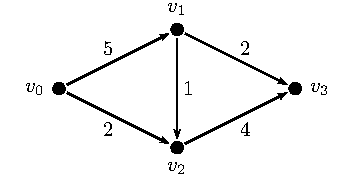
\includegraphics{fig4_1}
\end{center}

Formulieren Sie für dieses Netzwerk die Aufgabe, einen Fluss maximaler Stärke zu finden, als ein lineares Programmierungsproblem.
\Aufgabe[ (Energieflussprobleme mit Kosten)]{P3}
Für das Netzwerk aus Aufgabe P2 seien zusätzlich zu den Kapazitäten auch noch Kosten für jede Kante gegeben:

\begin{center}
 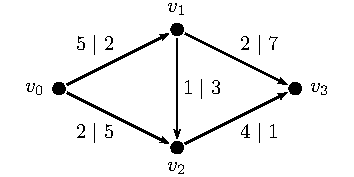
\includegraphics{fig4_2}
\end{center}

Gefragt ist nach einem \textit{kostenminimalen Fluss} der Stärke 4. Formulieren Sie diese Aufgabenstellung als LP-Problem.

\subsection*{Hausaufgaben bis zum 09.12.2020 (12:00 Uhr)}
\emph{Bitte reichen Sie Ihre Hausaufgaben in festen Zweier- oder Dreiergruppen bei Moodle ein. Bitte laden Sie ausschließlich \textbf{PDF-Dokumente} hoch, andernfalls können Ihre Hausaufgaben nicht korrigiert werden.}

\Aufgabe[ (Flussnetzwerke, 4 Punkte)]{H1}
\begin{enumerate}[a)]
	% Aufgabe H-1a
	\item Im nachfolgenden Flussnetzwerk bezeichne $v_0$ die Quelle, $v_7$ die Senke und die Zahlen an den Kanten bezeichnen die Kapazitäten.
	
	\begin{center}
    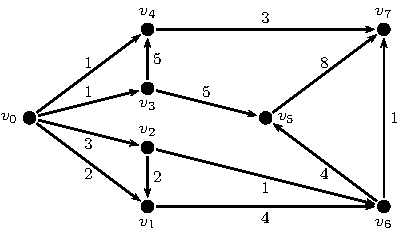
\includegraphics{fig4_3}
	\end{center}
	
	Formulieren Sie für dieses Netzwerk die Aufgabe, einen Fluss maximaler Stärke zu finden, als ein lineares Programmierungsproblem.
	
	% Aufgabe H-1b
	\item Für das folgende Netzwerk mit Quelle $v_0$ und Senke $v_6$ seien neben den Kapazitäten auch noch Kosten gegeben; die linke Zahl bezeichne die Kapazität, die rechte die Kosten einer Kante:
	
	\begin{center}
	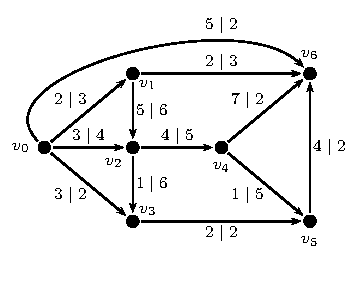
\includegraphics{fig4_4}
	\end{center}
	
	Gefragt ist nach einem kostenminimalen Fluss der Stärke 6. Formulieren Sie diese Aufgabenstellung als LP-Problem.
\end{enumerate}

\Aufgabe[ (Ganzzahlige LP-Probleme, 6 Punkte)]{H2}
\begin{enumerate}[a)]
	
	% Aufgabe H-2a
	\item Ein Personalchef habe für 2 offene Stellen 5 Bewerber, wobei aufgrund eines Eignungstests bekannt sei, welche Einarbeitungszeit $t_{ij}$ der Bewerber $i$ für die Stelle $j$ benötigt ($i=1,\ldots,5$ und $j=1,2$). Es sollen alle zwei Stellen besetzt werden -- drei Bewerber gehen leer aus. Die Einstellung soll so erfolgen, dass die Summe der Einarbeitungszeiten minimal ist. Formulieren Sie diese Aufgabe als ein binäres LP-Problem und veranschaulichen Sie die Fragestellung mithilfe eines bipartiten Graphen.
	
	% Aufgabe H-2b
	\item Es sei $G=(V,E)$ ein ungerichteter Graph mit Knotenmenge $V = \bigl\{ v_1,\ldots,v_n \bigr\}$ und Kantenmenge $E = \bigl\{ e_1,\ldots, e_m \bigr\}$. Eine Teilmenge $U$ der Knotenmenge heißt \textit{unabhängig}, falls keine zwei Knoten von $U$ durch eine Kante verbunden sind. Ein bekanntes, in der Informatik häufig betrachtetes Optimierungsproblem:
	\begin{equation}
	\tag{$\star$}
	\text{Finde in $G$ eine unabhängige Menge $U$, die möglichst viele Knoten enthält.}
	\end{equation}
	
	Formulieren Sie das Problem ($\star$) für den unten abgebildeten Graphen $G$ als ein binäres LP-Problem.
	
	\begin{center}
		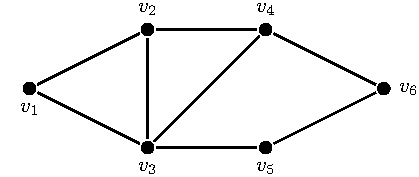
\includegraphics{fig4_5}
	\end{center}
	
	\textbf{Hinweis}: Für jeden Knoten $v_i$ ist eine Variable $x_i$ zu betrachten und für jede Kante ist eine Nebenbedingung zu formulieren.
	
	
	% Aufgabe H-2c
	\item Formulieren Sie das binäre Problem aus b) in ein ganzzahliges lineares Programmierungsproblem (ILP-Problem) um. Wie lautet die LP-Relaxation dieses Problems?
\end{enumerate}
\end{document}
